\documentclass[tikz,border=3.14mm]{standalone}
\usetikzlibrary{arrows.meta}
\begin{document}
  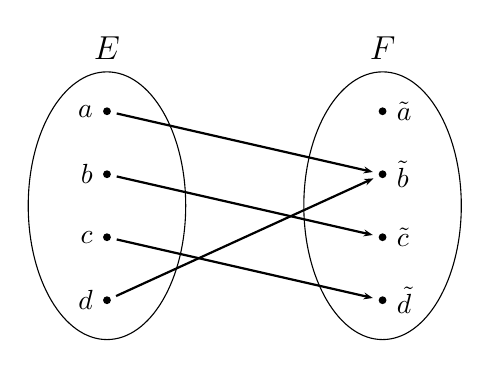
\begin{tikzpicture}[
      >={Stealth[scale=0.5]},
      bullet/.style={
        fill=black,
        circle,
        inner sep=1pt
      },
      projection/.style={
        ->,
        thick,
        shorten <=2pt,
        shorten >=2pt
      },
    ]

    \draw (0, 0) circle [x radius=1, y radius=1.7];
    \node [bullet, label=left:\(   a  \)] (a) at (0,1.2) {};
    \node [bullet, label=left:\(   b  \)] (b) at (0,0.4) {};
    \node [bullet, label=left:\(   c  \)] (c) at (0,-0.4) {};
    \node [bullet, label=left:\(   d  \)] (d) at (0,-1.2) {};
    \node[font=\large] (E) at (0, 2) {\(E\)};

    \begin{scope}[xshift=3.5cm]
      \draw (0, 0) circle [x radius=1, y radius=1.7]; 
      \node [bullet, label=right:\(    \tilde{a}     \)] (w) at (0,1.2) {};
      \node [bullet, label=right:\(    \tilde{b}     \)] (x) at (0,0.4) {};
      \node [bullet, label=right:\(    \tilde{c}     \)] (h) at (0,-0.4) {};
      \node [bullet, label=right:\(    \tilde{d}     \)] (v) at (0,-1.2) {};
      \node[font=\large] (F) at (0, 2) {\(F\)};
    \end{scope}

    \draw [projection] (a) -- (x);
    \draw [projection] (b) -- (h);
    \draw [projection] (c) -- (v);
    \draw [projection] (d) -- (x);
  \end{tikzpicture}
\end{document}